\section{Experimentación}

\subsection{Análisis de convergencia de PageRank}
%Imagen 1
\begin{wrapfigure}{r}{0.6\textwidth}
  \vspace{-20pt}
  \begin{center}
    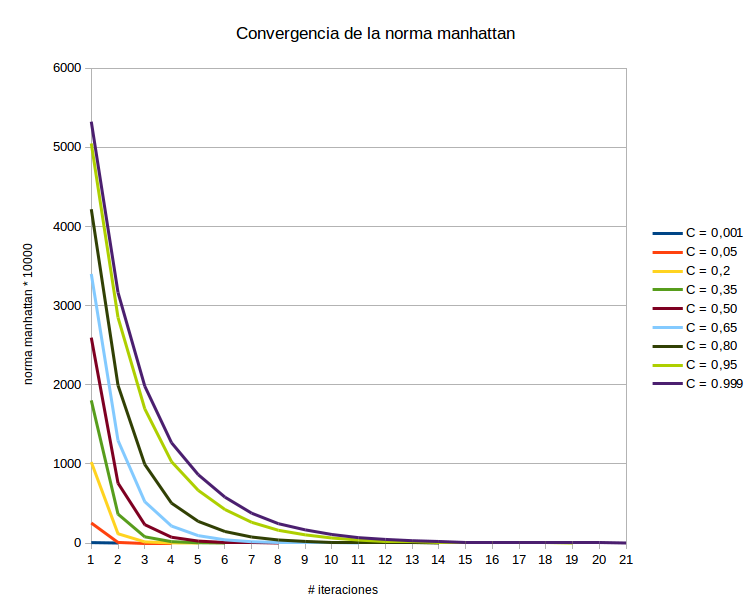
\includegraphics[scale= 0.6]{imagenes/convergencia1.png}
  \end{center}
  \vspace{-20pt}
   \caption{Con tantas páginas y tantos links.}
  \vspace{-10pt}
  \label{fig:img1}
\end{wrapfigure}

Para poder analizar la convergencia de PageRank realizamos mediciones de la cantidad de iteraciones que realiza el método de la potencia para el algoritmo, que termina cuando la norma de Manhattan es menor que un determinado valor muy cercano a 0.\\

Usamos tres instancias generadas al azar: La primera de 1000 páginas y 3000 links, la segunda de la misma cantidad de páginas pero 10000 links y la tercera de 500 páginas y 150000 links.\\

Nos interesa ver qué hace que el algoritmo termine en una menor cantidad de pasos y qué relación hay entre ese número y el valor de $c$. Ejecutamos $PageRank$ para cada instancia con una tolerancia fija de 0,00001, variando el valor del $c$ desde 0,001 hasta 0,999. Cada gráfico corresponde a los resultados obtenidos para una instancia distinta.\\



%Imagen 2
\begin{figure}[h]
  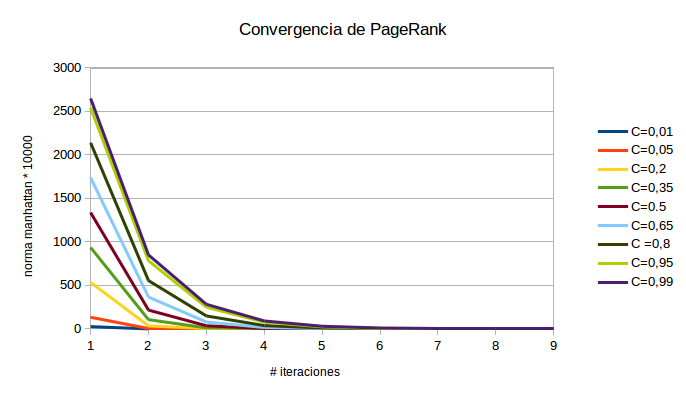
\includegraphics[scale= 0.6]{imagenes/convergencia2.png}
   \caption{Con tantas páginas y tantos links.}
  \label{fig:img1}
\end{figure}


\newpage

%Imagen 3
\begin{wrapfigure}{r}{0.6\textwidth}
  \vspace{-20pt}
  \begin{center}
    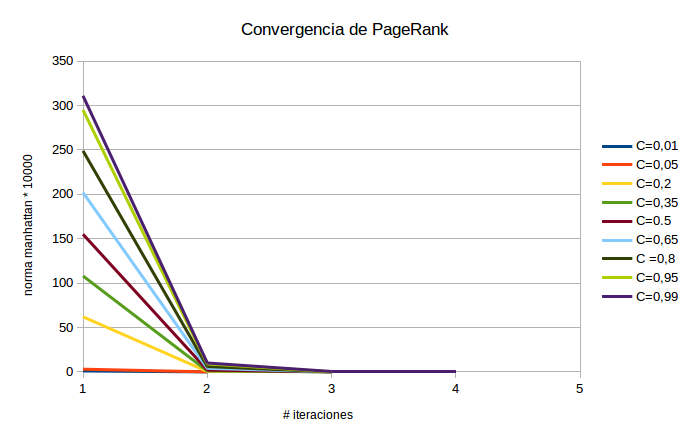
\includegraphics[scale= 0.6]{imagenes/convergencia3.png}
  \end{center}
  \vspace{-20pt}
   \caption{Con tantas páginas y tantos links.}
  \vspace{-10pt}
  \label{fig:img1}
\end{wrapfigure}

Mirando cada gráfico por separado podemos ver que la cantidad de iteraciones del algoritmo disminuye mientras más chico sea el valor de $c$, independientemente de que tan esparsa sea la matriz de links. 
Si comparamos los tres gráficos, vemos que las normas son mas chicas y el algoritmo converge más rápidamente mientras mas completa (menos esparsa) sea la matriz de links.\\



%% FALTA ANALISIS DE POR QUE PASA ESTO %%

%%%%%%%%%%%%%%%%%%%%%%%%%%%%%%%%%%%%%%%%%%%%%%%%%%%%%%%%%%%%%%%%%%%%%%%%%%%%%%%%%%%%%


Para ver como se comporta el algoritmo de $PageRank$ y comparar los resultados con los de $IN-DEG$, proponemos los siguientes ejemplos pequeños. Los grafos representan las páginas web y los link entre ellas, y las tablas muestran los resultados obtenidos de cada algoritmo.\\

%% ACA VAN LAS 6 IMAGENES DE GRAFOS , cada una junto a la tabla de resultados %%

%% ACA EL ANALISIS DE LOS RESULTADOS %%


\subsection{Análisis temporal de PageRank}

Para evaluar los tiempos del algoritmo PageRank con la estructura de matriz Vector que implementamos, generamos archivos de entradas de diferentes grafos. Son grafos generados aleatoriamente con cantidad de nodos desde 10 a 1000 y distintas cantidades de ejes de 10 a 1000. 
Ejecutamos el algoritmo para cada estructura y para cada uno de estos archivos de entrada. El siguiente gráfico muestra el tiempo obtenido en milisegundos dividido por la función $n^{2}$.\\


\begin{figure}[h]
  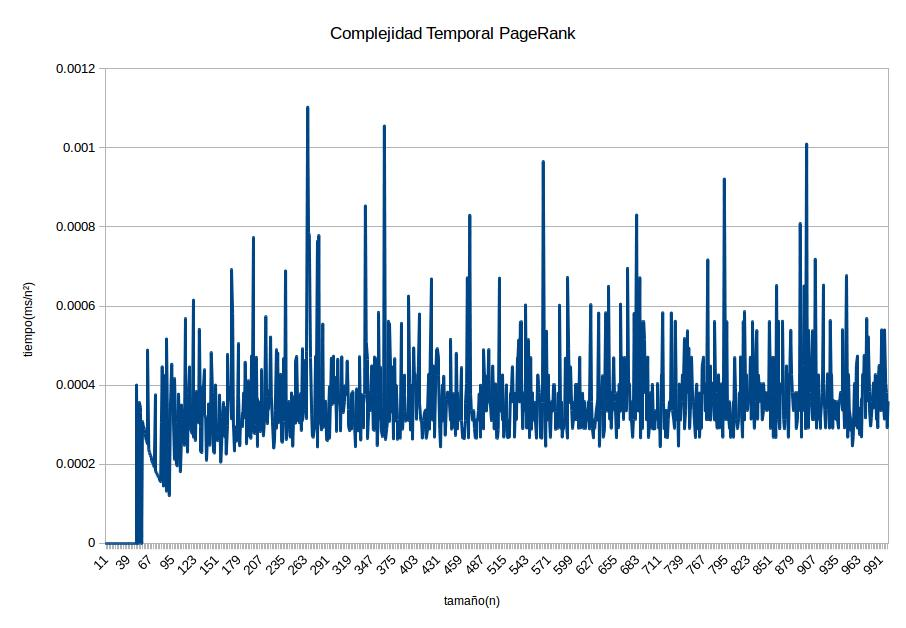
\includegraphics[scale= 0.4]{imagenes/complejidad-temporal-pagerank.png}
   \caption{Gráfico que representa el tiempo de corrida de PageRank con la estructura de datos Vector.}
  \label{fig:img1}
\end{figure}

El gráfico resultante es el de una función constante, lo que nos lleva a concluir que el algoritmo tiene una complejidad similar a O($n^{2}$).

\subsection{Comparación de performance del algoritmo sobre las distintas estructuras de datos}

El siguiente grafo detalla los resultados temporales de haber corrido instancias para PageRank con las estructuras de datos DOK, CSR y Vector.

\begin{figure}[h]
  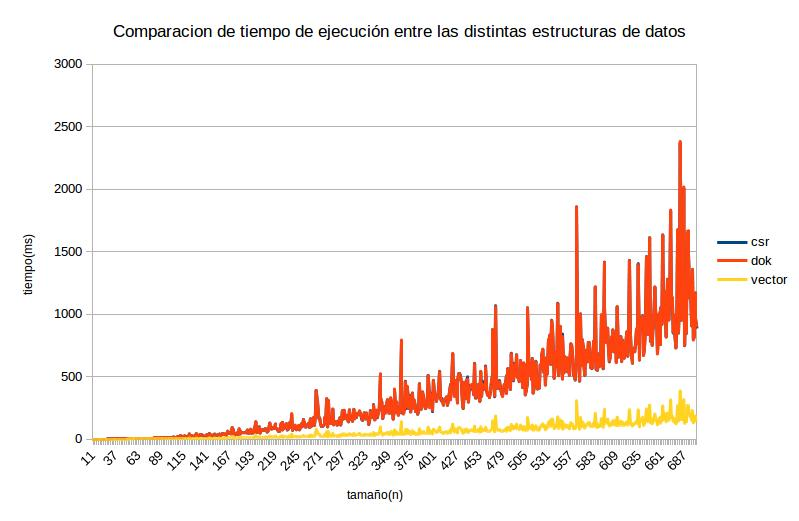
\includegraphics[scale=0.4]{imagenes/comparacion-tiempo-ejecucion-csr-dok-vector.png}
   \caption{Gráfico que representa el tiempo de corrida de PageRank con distintas estructuras de datos.}
  \label{fig:img1}
\end{figure}

Pudimos observar que CSR fue el más rápido de los 3, mientras que DOK es el más lento. A pesar de que tanto para CSR como DOK implementamos algoritmos más eficientes de multiplicación tanto para un escalar como para un vector, DOK resultó el más lento. \\

Creemos que esto se debe a la implementación interna de $map$ que está implementado sobre un Black-Red-tree. Tanto para multiplicar por un escalar como por un vector, iteramos por la estructura del mismo, de forma tal de aprovechar la esparcidad de la matriz y multiplicar sólo los elementos no nulos. En principio no encontramos una razón por la cual una implementación fuera mejor que la otra en cuanto a la forma de multiplicar desde el punto de vista algoritmico. Creemos que la razón radica en que, al iterar sobre los elementos de map se está haciendo una búsqueda binaria del próximo elemento en cada paso, dando como resultado que la complejidad de la operación no fuese $\mathcal{O}(nnz)$ sino $\mathcal{O}(nnz\log{}nnz)$ \\

Lo que nos resultó sorpresivo fue que incluso Vector tuvo una mejor performance que DOK, a pesar de que la complejidad de Vector para las operaciones anteriormente mencionadas es del orden cuadrático. Para este caso no pudimos obtener un resultado concluyente de por qué sucede esto. Una suposición a priori sugiere que se deba a optimizaciones realizadas por el compilador, explotando el hecho que Vector tenga todos sus elementos contiguos, disminuyendo así su tiempo de acceso. Sin embargo tal hipótesis excede nuestro análisis.

